\documentclass{article}  % Define la clase del documento.

% Paquetes de idioma y codificación
\usepackage[utf8]{inputenc}
\usepackage[T1]{fontenc}
\usepackage[spanish]{babel}  % Ajusta el idioma del documento a español.
\usepackage{tabularx}  % Permite la creación de tablas con ancho ajustable.

\usepackage{caption}
\usepackage{subcaption}

% Paquete de geometría para configurar márgenes y tamaño de papel
\usepackage[letterpaper, margin=3cm]{geometry}

% Paquetes de tipografía
\usepackage{mathptmx}    % Usa Times New Roman como fuente.
\usepackage{microtype}   % Mejora la justificación del texto.

% Paquetes para manejo de colores y gráficos
\usepackage{xcolor}      % Define y utiliza colores.
\usepackage{graphicx}    % Permite la inserción de imágenes.
\usepackage{tikz}        % Creación de gráficos vectoriales.

% Configuración de enlaces y referencias cruzadas
\usepackage{hyperref}
\hypersetup{
    colorlinks   = true,
    linkcolor    = darkblue,
    citecolor    = black,
    filecolor    = blue,
    urlcolor     = blue
}

\usepackage{media9} % Permite la inserción de multimedia.

% Paquetes para la mejora visual de tablas y figuras
\usepackage{booktabs}    % Para tablas de alta calidad.
\usepackage{float}       % Controla la posición de figuras y tablas.

% Paquete para la personalización de códigos fuente
\usepackage{listings}
\lstset{
    literate=
    {á}{{\'a}}1 {é}{{\'e}}1 {í}{{\'i}}1 {ó}{{\'o}}1 {ú}{{\'u}}1
    {Á}{{\'A}}1 {É}{{\'E}}1 {Í}{{\'I}}1 {Ó}{{\'O}}1 {Ú}{{\'U}}1
    {ñ}{{\~n}}1 {Ñ}{{\~N}}1 {ü}{{\"u}}1 {Ü}{{\"U}}1,
    backgroundcolor=\color{backcolour},
    commentstyle=\color{codegreen},
    keywordstyle=\color{codepurple},
    numberstyle=\tiny\color{codegray},
    stringstyle=\color{red},
    basicstyle=\ttfamily\small,
    breakatwhitespace=false,
    breaklines=true,
    captionpos=b,
    keepspaces=true,
    numbers=left,
    numbersep=5pt,
    showspaces=false,
    showstringspaces=false,
    showtabs=false,
    tabsize=2,
    language=TeX,
    morecomment=[l]\#,
    frame=single,
    rulecolor=\color{black}
}

% Definición de colores al estilo Visual Studio Code
\definecolor{darkblue}{rgb}{0.0, 0.0, 0.55}  % Enlaces
\definecolor{codegreen}{rgb}{0.25, 0.49, 0.48}  % Comentarios
\definecolor{codegray}{rgb}{0.5, 0.5, 0.5}  % Números y anotaciones
\definecolor{codepurple}{rgb}{0.58, 0, 0.82}  % Palabras clave
\definecolor{backcolour}{rgb}{0.95, 0.95, 0.92}  % Fondo de código

% Configuraciones de párrafo y matemáticas
\usepackage{amsmath}
\usepackage{parskip}    % Espaciado entre párrafos.
\usepackage{ragged2e}   % Justificación mejorada.
\usepackage{multicol}

% Configuración de secciones y encabezados
\usepackage{titlesec}
\titleclass{\part}{top} % Make part like a class
\titleformat{\part}[display]
  {\normalfont\huge\bfseries\centering}{\thepart}{40pt}{\Huge}
\titlespacing*{\part}{0pt}{-60pt}{10pt}
\titleformat{\part}
  {\normalfont\huge\bfseries}{}{0pt}{}

% Asegúrate de usar esto para mantener el estilo en las páginas de las partes
\titleformat{\part}[display]
  {\normalfont\huge\bfseries}{}{0pt}{}
  [\thispagestyle{fancy}] % Aplica el estilo fancy a las páginas de las partes

% Configuración de encabezados y pies de página personalizados
\usepackage{fancyhdr}
\pagestyle{fancy}
\fancyhf{}
\fancyhead[L]{\raisebox{0.20cm}{\textbf{Dynamics of structures}}}
\fancyhead[R]{\raisebox{0.1cm}{
\includegraphics[width=0.25\linewidth]{LOGO_UNIVERSIDAD.jpg}}}
\fancyhead[C]{\rule{\textwidth}{0.6pt}}
\fancyfoot[C]{\rule{\textwidth}{0.6pt}}
\fancyfoot[R]{\raisebox{-1.5\baselineskip}{\thepage}}
\renewcommand{\headrulewidth}{0pt}
\renewcommand{\footrulewidth}{0pt}

% Configuración avanzada de geometría
\geometry{
  top=3.5cm, % Aumenta el espacio en la parte superior para subir el encabezado
  bottom=2.5cm,
  headheight=2.5cm % Aumenta la altura del encabezado si es necesario
}

% Configuracion de bibliografia
\usepackage{natbib}
\bibliographystyle{unsrtnat}  % Puedes cambiarlo por `unsrtnat`, `abbrvnat`, etc.

\begin{document}
%----------------------------------------------------------------------------------------
% PORTADA
%----------------------------------------------------------------------------------------
\begin{titlepage}%Inicio de la carátula, solo modificar los datos necesarios
\newcommand{\HRule}{\rule{\linewidth}{0.5mm}} 
\center 
%----------------------------------------------------------------------------------------
%	ENCABEZADO
%----------------------------------------------------------------------------------------

\includegraphics[width=10cm]{LOGO_UNIVERSIDAD.jpg}\\ % Si esta plantilla se copio correctamente, va a llevar la imagen del logo de la facultad.OBS: Es necesario incluir el paquete: graphicx
\vspace{3cm}
%----------------------------------------------------------------------------------------
%	SECCION DEL TITULO
%----------------------------------------------------------------------------------------
\HRule \\[0.4cm]
{ \huge \bfseries Dynamics of structures}\\[0.4cm] % Titulo del documento
{ \huge \bfseries Laboratory 1: Single Degree of Freedom System}\\[0.4cm] % Titulo del documento
\HRule \\[1.5cm]
 \vspace{5cm}
%----------------------------------------------------------------------------------------
%	SECCION DEL AUTOR
%----------------------------------------------------------------------------------------
\begin{flushright}
  { \textbf{Professor:}\\
  Francisco Hernandez\\
  \textbf{Assistance:}\\
  Gastón Parra\\
  \textbf{Students:} \\
  Bernardo Caprile\\
  Pedro Valenzuela\\
  Felipe Vicencio\\
  Lukas Wolff\\
}
\end{flushright}
\vspace{1cm}
%----------------------------------------------------------------------------------------
%	SECCION DE LA FECHA
%----------------------------------------------------------------------------------------
{\large \textbf{\today}}\\[2cm] % El comando \today coloca la fecha del dia, y esto se actualiza con cada compilacion, en caso de querer tener una fecha estatica, reemplazar el \today por la fecha deseada
\end{titlepage}

\newpage
\thispagestyle{empty} % Deshabilita el número de página en la página del índice

%----------------------------------------------------------------------------------------
%  INDICE
%----------------------------------------------------------------------------------------
%\newpage
%\thispagestyle{empty} % Deshabilita el número de página en la página del índice
%\tableofcontents
%\thispagestyle{plain} % Deshabilita el encabezado en la página del índice
%\thispagestyle{empty} % Deshabilita el número de página en la página del índice
%\newpage

%\newpage
%\thispagestyle{empty}
%\listoffigures 
%\thispagestyle{plain} % Deshabilita el encabezado en la página del índice %
%\thispagestyle{empty}
\newpage
%----------------------------------------------------------------------------------------
%ACÁ EMPIEZA EL INFORME
\setcounter{page}{1}
%----------------------------------------------------------------------------------------

\section{Introduction}
To understand the dynamic behavior of complex structures with multiple degrees of freedom, it is essential to first study single degree of freedom (SDOF) systems. These simplified models serve as the foundation for analyzing structural response under dynamic loading. In this laboratory experiment, we aim to determine the natural period and damping ratio of an SDOF system using various experimental methods. This includes performing a pull-back test and applying the logarithmic decrement technique to estimate damping characteristics. Additionally, the system is subjected to harmonic base excitation to identify its natural frequency and evaluate resonance behavior. The results obtained experimentally are then compared to those derived from an analytical model, providing insight into the accuracy and limitations of both approaches. This foundational knowledge is critical for the design and analysis of real-world engineering structures subjected to dynamic forces.


\begin{figure}[h]
  \centering
  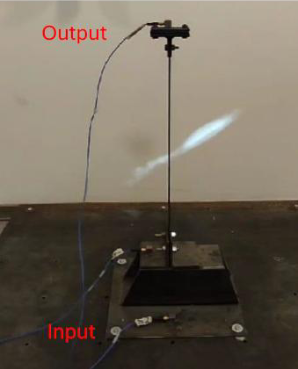
\includegraphics[width=0.5\textwidth]{GRAFICOS/SDOF_picture.PNG}
  \caption{Single Degree of Freedom System.}
  \label{fig:sdof}
\end{figure}
  
The experimental structure used to model the single degree of freedom (SDOF) system consists of a vertical flexible rod rigidly fixed at its base. At the top of the rod, a small mass is attached, allowing for lateral motion when the system is excited. The input motion is applied at the base (as indicated by the “Input” label in the figure), while the output is measured at the top mass using a acceleration sensor (labeled “Output”). This setup simulates the behavior of an idealized SDOF system by allowing one mode of vibration in the lateral direction, the mass, the flexural stiffness of the rod, and the system's inherent damping.




\newpage

\section{Theoretical Background}

\subsection{Natural Frequency}
The natural frecuency of a system is the rate at which the body oscillates when it is distrurbed without any damping or external forces acting on it. This parameter is crucial in understanding the dynamic behavior of structures, as it determines how the system will respond to external excitations. The natural frequency can be calculated using the following formula:
\begin{equation}
\omega_n = \sqrt{\frac{k}{m}}
\end{equation}
Where:
\begin{itemize}
  \item $\omega_n$ = natural frequency (rad/s)
  \item $k$ = stiffness of the system (N/m)
  \item $m$ = mass of the system (kg)
\end{itemize}

One of the important aspects of the natural frequency is that it is inversely proportional to the mass of the system. This means that as the mass increases, the natural frequency decreases, and vice versa. This relationship is crucial in designing structures to ensure they can withstand dynamic loads without resonating at their natural frequency.

\subsection{Damping Ratio}
The damping ratio is a parameter that has the effect of reduciong the oscillations of a system over time. In physical systems, damping is caused by energy dissipation mechanisms such as friction, air resistance or dampers. The damping ratio is defined as the ratio of the actual damping to the critical damping, and it can be calculated using the following formula:
\begin{equation}
\beta = \frac{c}{2\sqrt{mk}}
\end{equation}
Where:
\begin{itemize}
  \item $\beta$ = damping ratio (dimensionless)
  \item $c$ = damping coefficient (N.s/m)
  \item $k$ = stiffness of the system (N/m)
  \item $m$ = mass of the system (kg)
\end{itemize}

\subsection{Logarithmic Decrement}
The logarithmic decrement is a measure of the rate at which the amplitude of oscillations decreases over time in a damped system. It is defined as the natural logarithm of the ratio of two successive amplitudes, and it can be calculated using the following formula:

\begin{equation}
\delta = \frac{1}{n} \ln \left( \frac{x_0}{x_n} \right)
\end{equation}
Where:
\begin{itemize}
  \item $\delta$ = logarithmic decrement (dimensionless)
  \item $x_0$ = amplitude of the first oscillation (m)
  \item $x_n$ = amplitude of the n-th oscillation (m)
  \item $n$ = number of oscillations (dimensionless)
\end{itemize}

With this parameter, we can determine the damping ratio of the system using the following formula:

\begin{equation}
\beta = \frac{\delta}{\sqrt{4\pi^2 + \delta^2}}
\end{equation}
Where:
\begin{itemize}
  \item $\delta$ = logarithmic decrement (dimensionless)
  \item $\beta$ = damping ratio (dimensionless)
\end{itemize}

\subsection{Harmonic base excitation}
The harmonic base excitation is a phenomenon that occurs when a system is subjected to a periodic force at its base. This type of excitation is key in understanding the dynamic behavior of structures, due to every structure suffers from this type of excitation. 

\subsection{Transmissibility}
Transmissibility is a measure of how much the input motion is transmitted to the output of a system. It is defined as the ratio of the output response to the input response, and it can be calculated using the following formula:
\begin{equation}
TR = \frac{\ddot{X}}{\ddot{X_g}} = \sqrt{\frac{1+(2 \beta (\bar{\omega}/\omega_n)^2}{(1 - \frac{\bar{\omega}^2}{\omega_n^2})^2 + (2\beta\frac{\bar{\omega}}{\omega_n})^2}} 
\end{equation}
Where:
\begin{itemize}
  \item $TR$ = transmissibility (dimensionless)
  \item $\ddot{X_g}$ = output acceleration (m/s$^2$) (acceleration of the base) 
  \item $\ddot{X}$ = input acceleration (m/s$^2$) (acceleration of the mass)
  \item $\bar{\omega}$ = frequency of the input motion (rad/s)
  \item $\omega_n$ = natural frequency of the system (rad/s)
  \item $\beta$ = damping ratio (dimensionless)
\end{itemize}

Due to the transmissibility, if the excitation frecuency is much smaller than the natural frequency of the system ($\bar{\omega} < \omega_n$), the transmissibility is close to 1, which means that the input motion is transmitted to the output with little amplification. On the other hand, if the excitation frequency is bigger to the natural frequency of the system ($\bar{\omega} > \omega_n$), the transmissibility is close to 0, which means that the input motion is transmitted to the output with null amplification. Finally, if the excitation frequency is equal to the natural frequency of the system ($\bar{\omega} = \omega_n$), the transmissibility is infinite, which means that the input motion is transmitted to the output with a high amplification. This phenomenon is known as resonance.

\subsection{Resonance}
Resonance is a phenomenon that occurs when the frequency of an external force matches the natural frequency of a system:

$$\omega_n = \bar{\omega}$$

For an undamped system the factor of amplification is infinite, which means that the system will oscillate indefinitely with increasing amplitude. In real systems, damping reduces the maximum amplitude of oscillations, but resonance can still lead to significant increases in amplitude. This means, if the resonance is not controlled, it can cause structural damage or failure. 

 


\end{document} 